\section{Why is Less More? Ablations on Data Diversity, Quality, and Quantity}
\label{sec:ablations}

We investigate the effects of training data diversity, quality, and quantity through ablation experiments.
We observe that, for the purpose of alignment, scaling up input diversity and output quality have measurable positive effects, while scaling up quantity alone might not.
% \mike{To me this paragraph doesn't quite answer the question in the section title. Maybe add a sentence like: "Therefore, we recommend focusing efforts on curating smaller, high quality alignment datasets, instead of large scale annotation."}

\paragraph{Experiment Setup}
We fine-tune a 7B parameter LLaMa model \cite{touvron2023llama} on various datasets, controlling for the same hyperparameters (Section~\ref{sec:training}).\footnote{While preliminary experiments show that it is possible to tune the 7B model with only 1,000 examples, we also found that using at least 2,000 examples improved stability in this setting.}
We then sample 5 responses for each test set prompt, and evaluate response quality by asking ChatGPT (GPT-3.5 Turbo) to grade the helpfulness of a response on a 1-6 likert scale (see Appendix~\ref{sec:gpt_annotation} for exact template).
We report the average score alongside a $p=0.95$ two-sided confidence interval.
% \omer{comment this out?} In hindsight, we find that this evaluation method is indeed sensitive to bad generations, but does not always differentiate between good and better responses.


\begin{figure}[t]
     \centering
     \begin{minipage}[t]{0.475\textwidth}
         \centering
         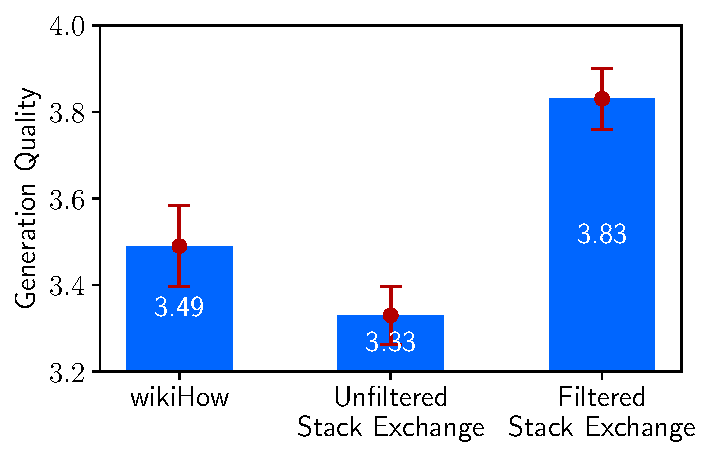
\includegraphics[width=\linewidth]{figs/quality_bar.pdf}
         \caption{Performance of 7B models trained with 2,000 examples from different sources. \textbf{Filtered Stack Exchange} contains diverse prompts and high quality responses; \textbf{Unfiltered Stack Exchange} is diverse, but does not have any quality filters; \textbf{wikiHow} has high quality responses, but all of its prompts are ``how to'' questions.}
         \label{fig:quality}
     \end{minipage}
     \hfill
     \begin{minipage}[t]{0.475\textwidth}
         \centering
         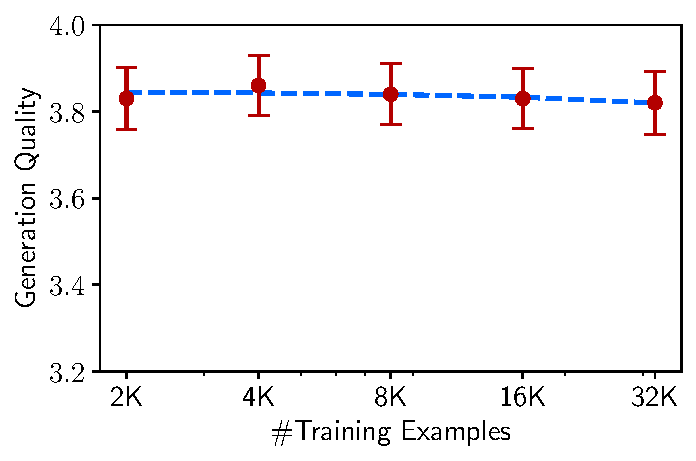
\includegraphics[width=\linewidth]{figs/quantity_se.pdf}
         \caption{Performance of 7B models trained with exponentially increasing amounts of data, sampled from (quality-filtered) Stack Exchange. Despite an up to 16-fold increase in data size, performance as measured by ChatGPT plateaus.}
         \label{fig:quantity}
     \end{minipage}
\end{figure}



% \begin{figure}[t]
%     \centering
%     \begin{minipage}{0.70\textwidth}
%         \centering
%         \begin{minipage}{\linewidth}
%             \centering
%             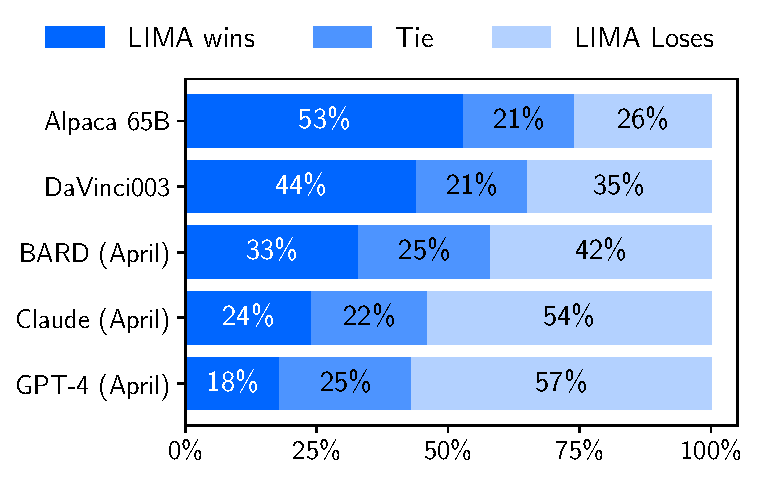
\includegraphics[width=\linewidth]{figs/human_eval.pdf}
%             % 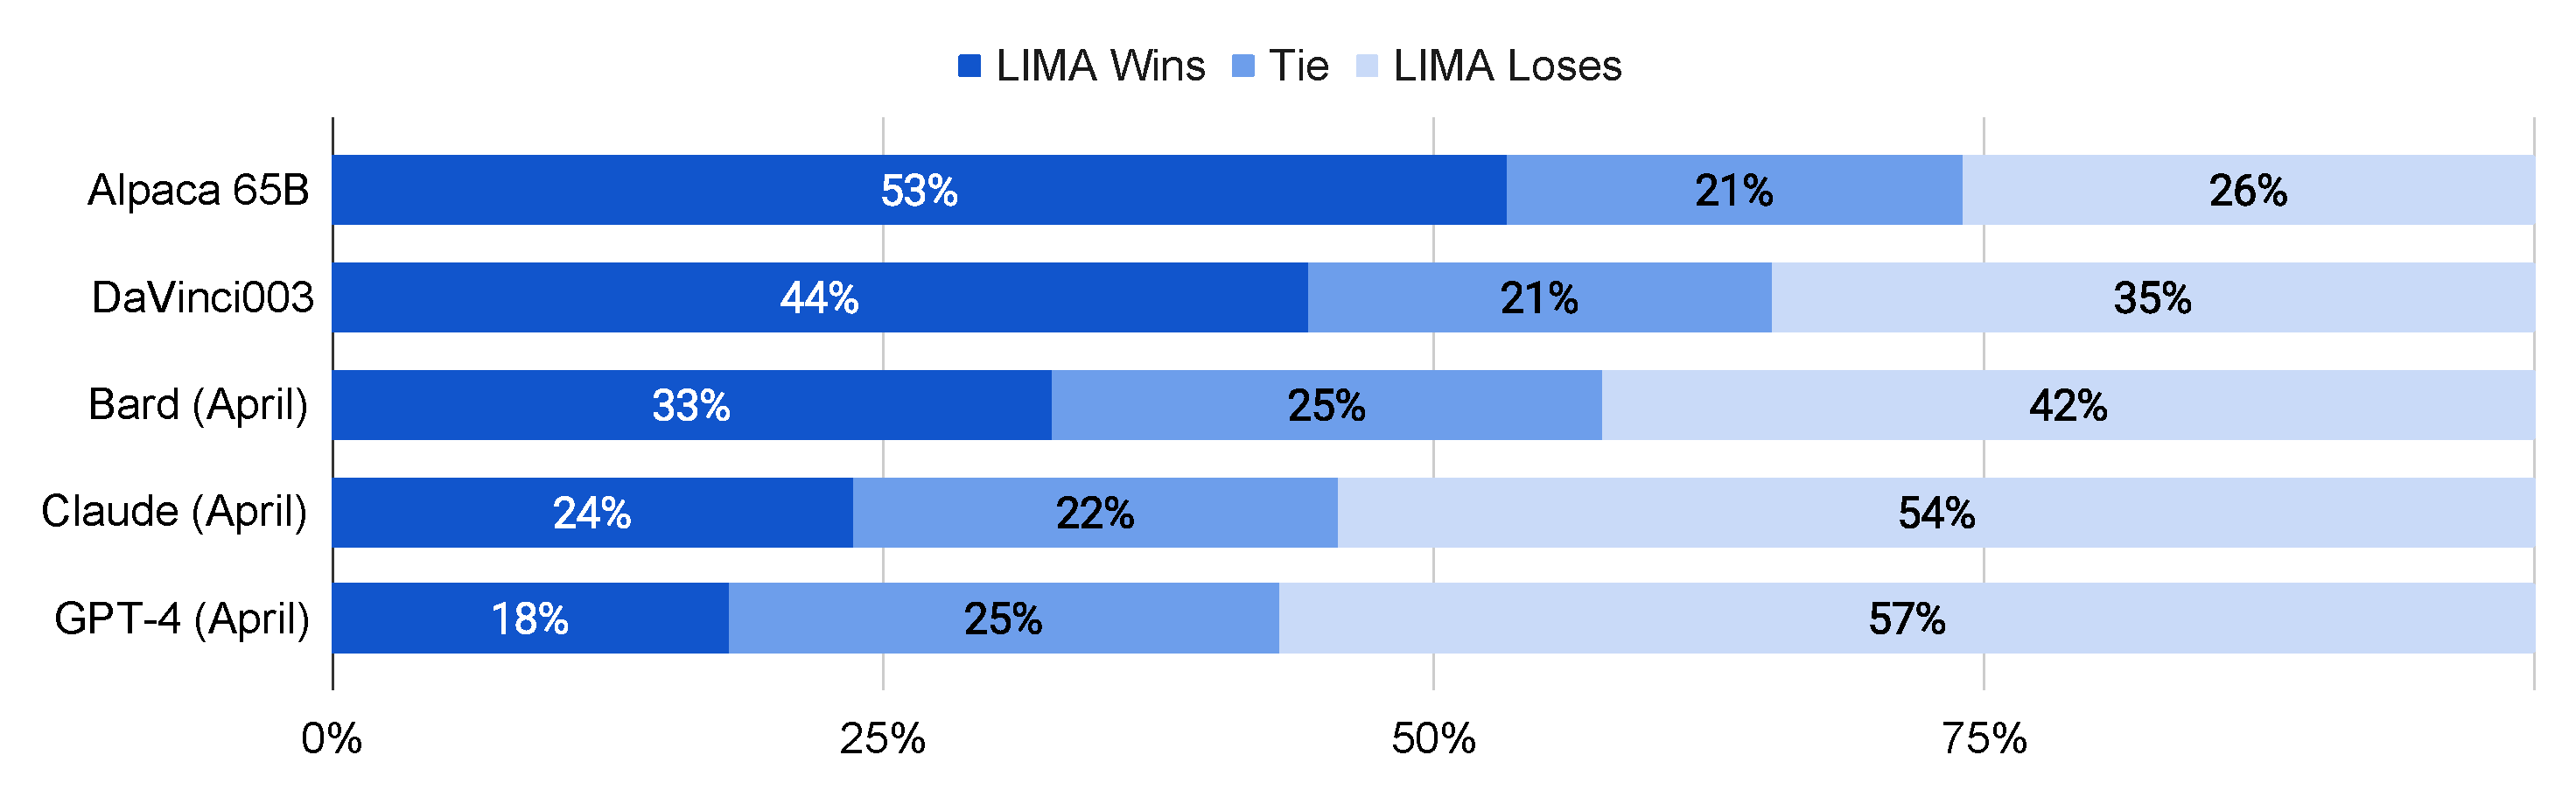
\includegraphics[width=\linewidth]{figs/gs_results_human.pdf}
%             \caption{Human preference evaluation, comparing LIMA to 5 different baselines across 300 test prompts.}
%             \label{fig:results_human}
%         \end{minipage}
        
%         \begin{minipage}{\linewidth}
%             \centering
%             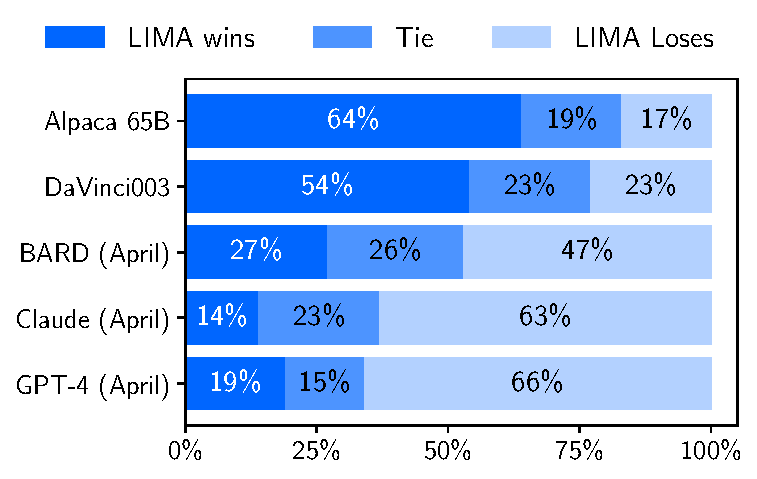
\includegraphics[width=\linewidth]{figs/gpt4_eval.pdf}
%             % 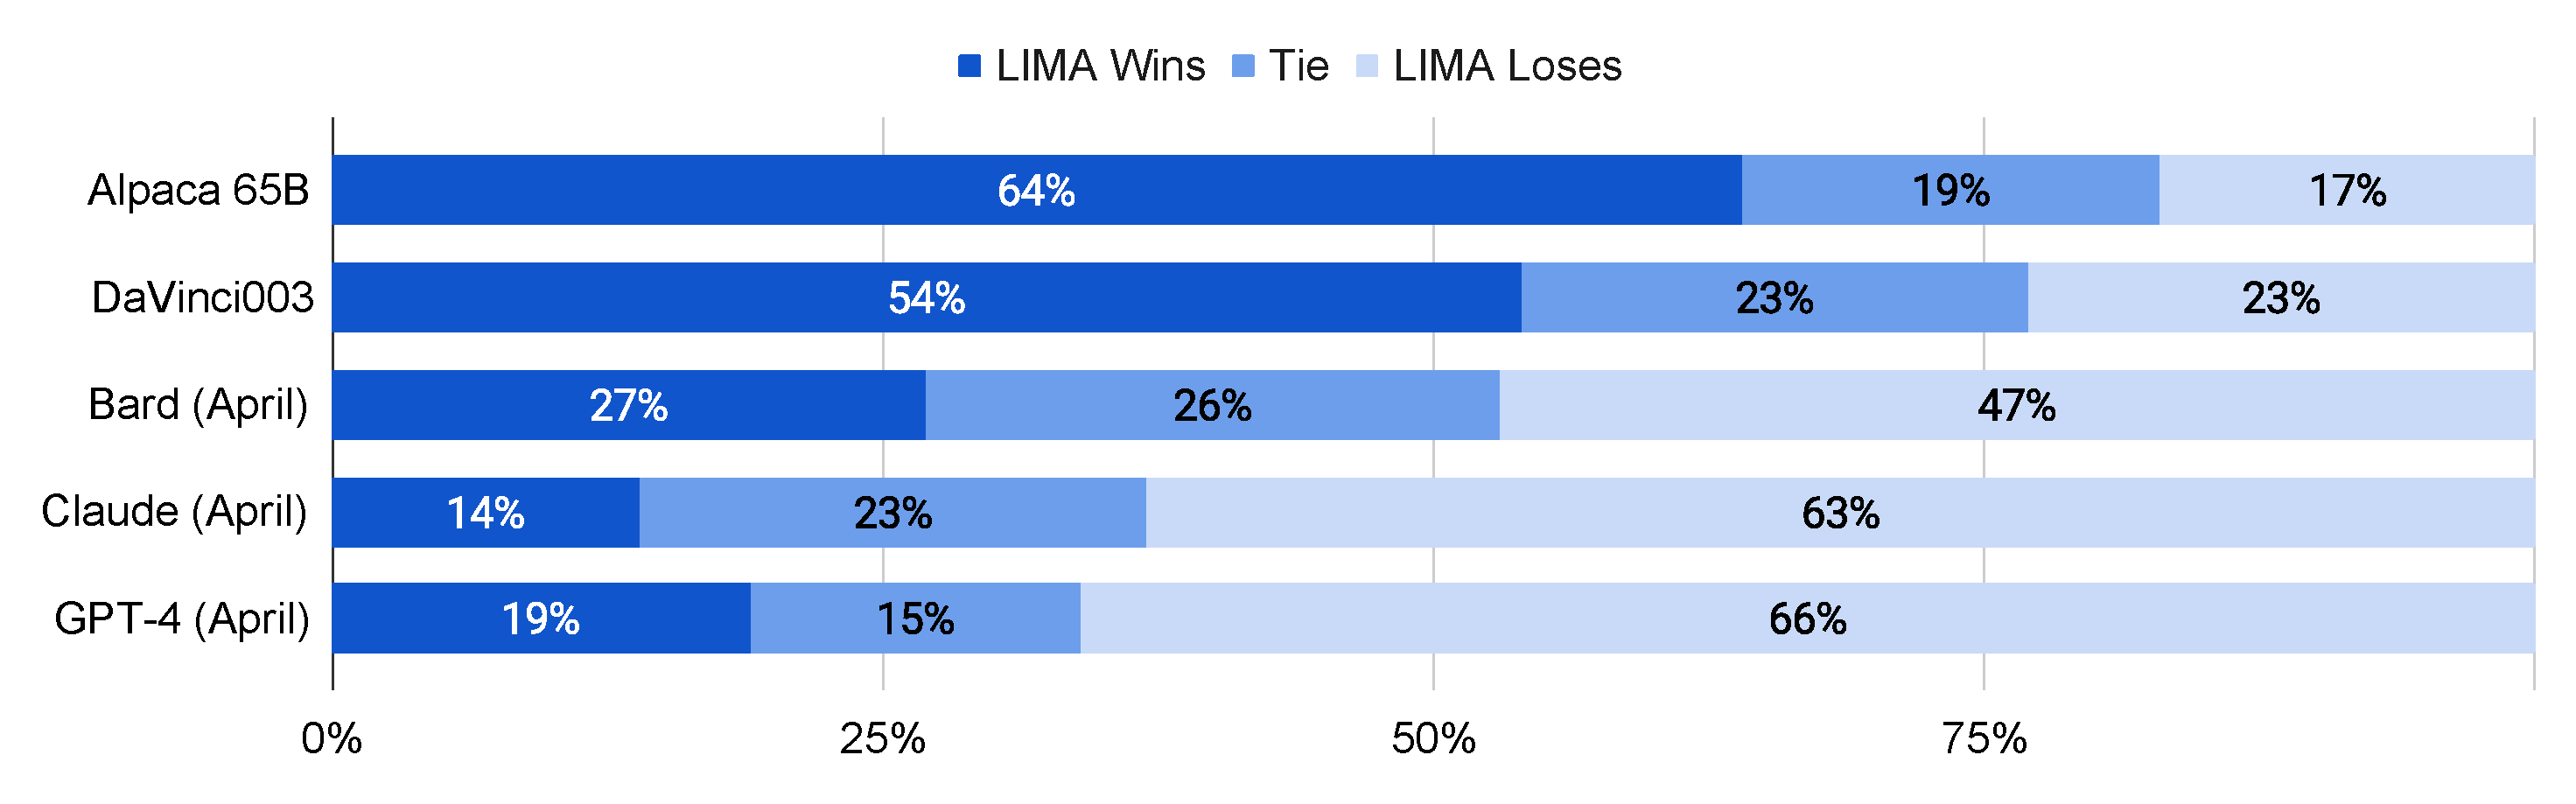
\includegraphics[width=\linewidth]{figs/gs_results_gpt4.pdf}
%             \caption{Preference evaluation using GPT-4 as the annotator, given the same instructions provided to humans.}
%             \label{fig:results_gpt4}
%         \end{minipage}
%     \end{minipage}
%     \hfill
%     \begin{minipage}{0.25\textwidth}
%         \centering
%         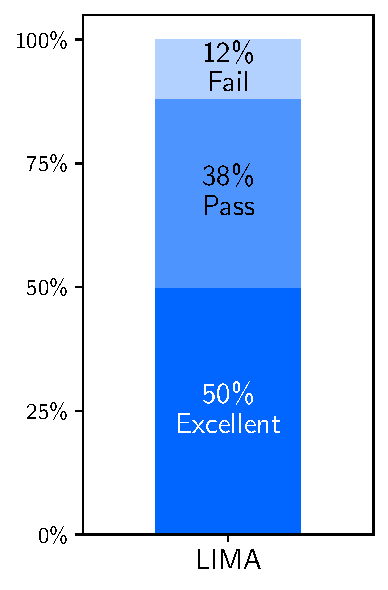
\includegraphics[width=\linewidth]{figs/analysis_bar.pdf}
%         % 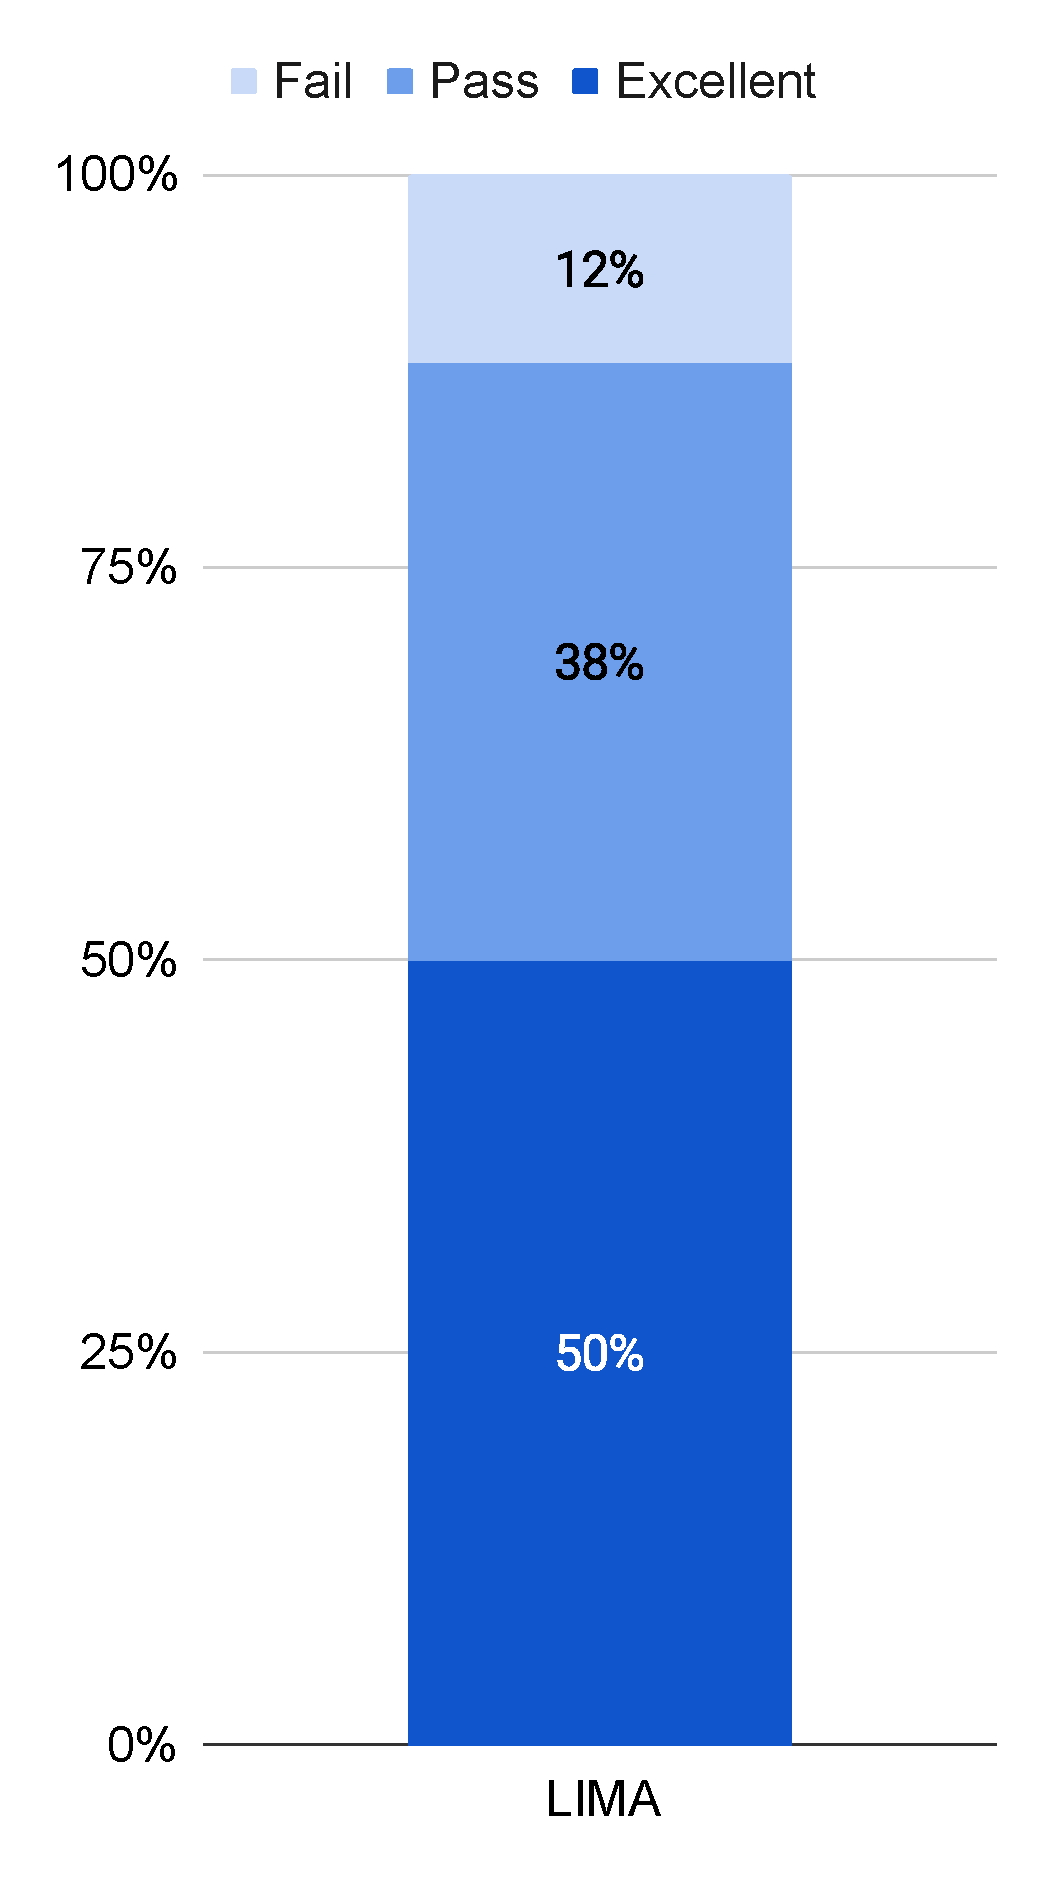
\includegraphics[width=\linewidth]{figs/gs_analysis.pdf}
%         \caption{Manual analysis of LIMA's response to 50 test prompts.}
%         \label{fig:analysis}
%     \end{minipage}
% \end{figure}



\paragraph{Diversity}
To test the effects of prompt diversity, while controlling for quality and quantity, we compare the effect of training on quality-filtered Stack Exchange data, which has \textit{heterogeneous} prompts with excellent responses, and wikiHow data, which has \textit{homogeneous} prompts with excellent responses.
While we compare Stack Exchange with wikiHow as a proxy for diversity, we acknowledge that there may be other conflating factors when sampling data from two different sources.
We sample 2,000 training examples from each source (following the same protocol from Section~\ref{sec:community_data}).
Figure~\ref{fig:quality} shows that the more diverse Stack Exchange data yields significantly higher performance.

\paragraph{Quality}
To test the effects of response quality, we sample 2,000 examples from Stack Exchange \textit{without} any quality or stylistic filters, and compare a model trained on this dataset to the one trained on our filtered dataset.
Figure~\ref{fig:quality} shows that there is a significant 0.5 point difference between models trained on the filtered and unfiltered data sources.

\paragraph{Quantity}
Scaling up the number of examples is a well-known strategy for improving performance in many machine learning settings.
To test its effect on our setting, we sample exponentially increasing training sets from Stack Exchange.
Figure~\ref{fig:quantity} shows that, surprisingly, doubling the training set does not improve response quality.
This result, alongside our other findings in this section, suggests that the scaling laws of alignment are not necessarily subject to \textit{quantity} alone, but rather a function of prompt \textit{diversity} while maintaining high quality responses.
